\chapter{Basic Documentation generated from README.md}
\label{app:basicDocs}

\begin{figure}[htp]
\centering
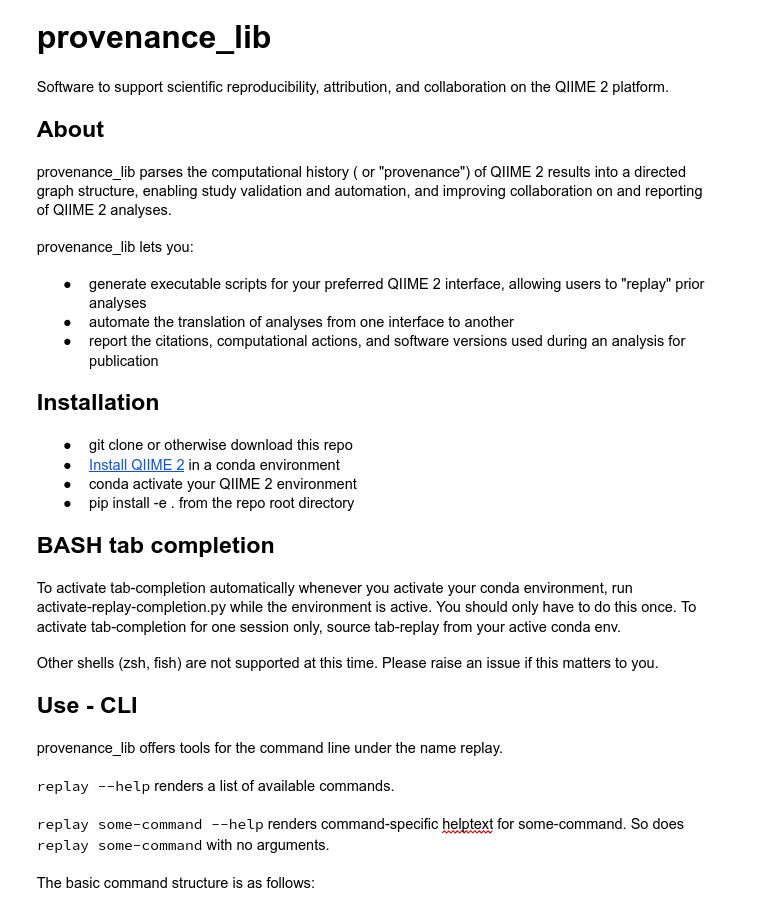
\includegraphics[width=.95\textwidth]{figures/AppA1.png}
\end{figure}

\begin{figure}[htp]
\centering
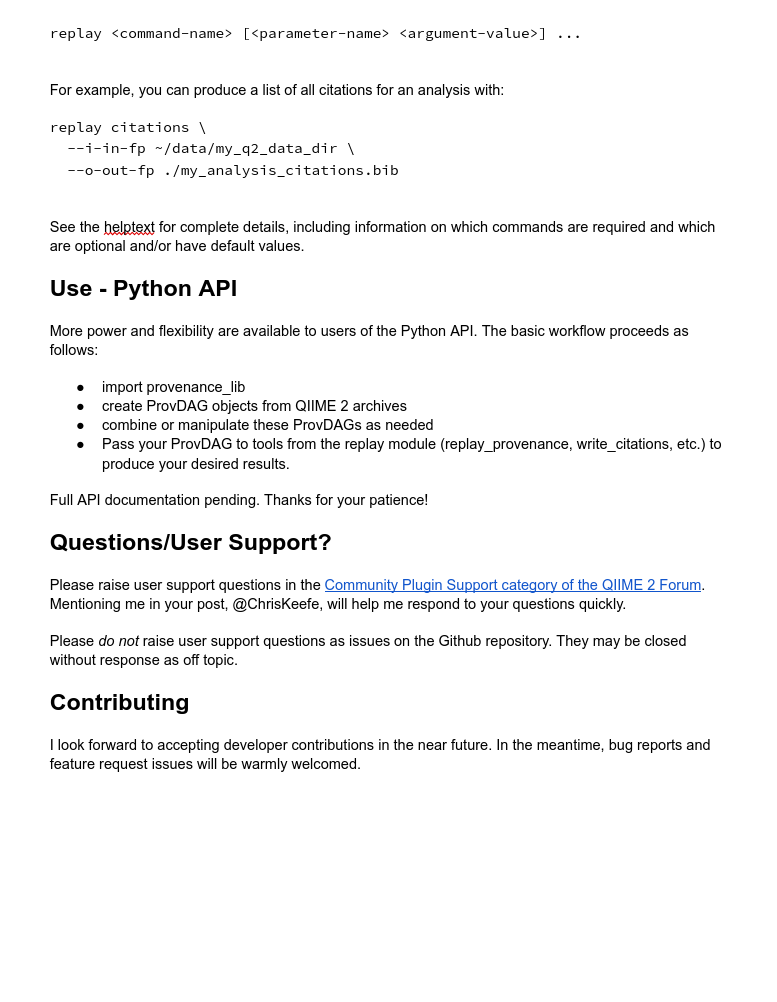
\includegraphics[width=\textwidth]{figures/AppA2.png}
\end{figure}

% \clearpage
% \hypertarget{provenance_lib}{%
% \section*{provenance\_lib}\label{provenance_lib}}
% 
% \noindent Software to support scientific reproducibility, attribution, and
% collaboration on the QIIME 2 platform.
% 
% \hypertarget{about}{%
% \subsection*{About}\label{about}}
% 
% \noindent provenance\_lib parses the computational history ( or ``provenance'') of
% QIIME 2 results into a directed graph structure, enabling study
% validation and automation, and improving collaboration on and reporting
% of QIIME 2 analyses. \\
% 
% \noindent provenance\_lib lets you: - generate executable scripts for your
% preferred QIIME 2 interface, allowing users to ``replay'' prior analyses
% - automate the translation of analyses from one interface to another -
% report the citations, computational actions, and software versions used
% during an analysis for publication
% 
% \hypertarget{installation}{%
% \subsection*{Installation}\label{installation}}
% 
% \begin{itemize}
% \tightlist
% \item
%   \texttt{git\ clone} or otherwise download this repo
% \item
%   \href{https://docs.qiime2.org/2021.11/install/}{Install QIIME 2} in a
%   conda environment
% \item
%   \texttt{conda\ activate} your QIIME 2 environment
% \item
%   \texttt{pip\ install\ -e\ .} from the repo root directory
% \end{itemize}
% 
% \hypertarget{bash-tab-completion}{%
% \subsection*{BASH tab completion}\label{bash-tab-completion}}
% 
% \noindent To activate tab-completion automatically whenever you activate your
% conda environment, run \texttt{activate-replay-completion.py} while the
% environment is active. You should only have to do this once. To activate
% tab-completion for one session only, \texttt{source\ tab-replay} from
% your active conda env. \\
% 
% \noindent Other shells (zsh, fish) are not supported at this time. Please raise an
% issue if this matters to you.
% 
% \hypertarget{use---cli}{%
% \subsection*{Use - CLI}\label{use---cli}}
% 
% \noindent provenance\_lib offers tools for the command line under the name
% \texttt{replay}. \\
% 
% \noindent \texttt{replay\ -\/-help} renders a list of available commands.
% 
% \noindent \texttt{replay\ some-command\ -\/-help} renders command-specific
% helptext for \texttt{some-command}. So does
% \noindent \texttt{replay\ some-command} with no arguments.
% 
% \noindent The basic command structure is as follows:
% 
% \begin{verbatim}
% replay <command-name> [<parameter-name> <argument-value>] ...
% \end{verbatim}
% 
% \noindent For example, you can produce a list of all citations for an analysis
% with:
% 
% \begin{verbatim}
% replay citations \
%   --i-in-fp ~/data/my_q2_data_dir \
%   --o-out-fp ./my_analysis_citations.bib
% \end{verbatim}
% 
% \noindent See the helptext for complete details, including information on which
% commands are required and which are optional and/or have default values.
% 
% \hypertarget{use---python-api}{%
% \subsection*{Use - Python API}\label{use---python-api}}
% 
% \noindent More power and flexibility are available to users of the Python API. The
% basic workflow proceeds as follows:
% \begin{itemize}
%     \item \texttt{import\ provenance\_lib}
%     \item create ProvDAG objects from QIIME 2 archives
%     \item combine or manipulate these ProvDAGs as needed
%     \item Pass your ProvDAG to tools from the \texttt{replay} module (\texttt{replay\_provenance}, \texttt{write\_citations}, etc.) to produce your desired results.
% \end{itemize}
% 
% \noindent Full API documentation pending. Thanks for your patience!
% 
% \hypertarget{questionsuser-support}{%
% \subsection*{Questions/User Support?}\label{questionsuser-support}}
% 
% \noindent Please raise user support questions in the
% \href{https://forum.qiime2.org/c/community-plugin-support/}{Community
% Plugin Support category of the QIIME 2 Forum}. Mentioning me in your
% post, @ChrisKeefe, will help me respond to your questions quickly. \\
% 
% \noindent Please \emph{do not} raise user support questions as issues on the
% Github repository. They may be closed without response as off topic.
% 
% \hypertarget{contributing}{%
% \subsection*{Contributing}\label{contributing}}
% 
% \noindent I look forward to accepting developer contributions in the near future.
% In the meantime, bug reports and feature request issues will be warmly
% welcomed.